\documentclass[11pt]{article}
% Font tiếng việt
\usepackage{fontspec}
\usepackage[vietnamese]{babel}

% Sử dụng bảng dài có thể ngắt trang, bạn cần thêm 2 gói này vào preamble
\usepackage{longtable}
\usepackage{ragged2e}


\usepackage{graphicx}
\usepackage{amsmath, amssymb, amsfonts, bm}
\usepackage{xcolor}
\usepackage{hyperref}
\usepackage{pifont}
\newcommand{\xmark}{\ding{55}}
\newcommand{\cmark}{\ding{51}}
\usepackage{array}
\usepackage{float}

\definecolor{codehighlight}{rgb}{0.95,0.95,0.92} % Using your backcolour


\hypersetup{
    colorlinks=true,
    linkcolor=blue,
    filecolor=magenta,
    urlcolor=red,
    pdftitle={Overleaf Example},
    pdfpagemode=FullScreen,
}

\setmainfont{Times New Roman}
% \setsansfont{Arial} % Not used in the final layout, can comment out
% \setmonofont{Courier New} % Not used in the final layout, can comment out


% Page layout
\setlength{\topmargin}{-.5in}
\setlength{\textheight}{9.25in}
\setlength{\oddsidemargin}{0in}
\setlength{\textwidth}{6.8in}

% No explicit title formatting needed as we'll place it manually
\usepackage{titling}
\setlength{\droptitle}{-10em} % Keep this to prevent default title spacing issues if using \maketitle later for other purposes

\renewcommand{\maketitle}{%
    \begin{center}
        \fontsize{18}{20}\selectfont\textbf{Tuần 1 - Tổng hợp kiến thức Buổi học số 1 và 2}\\[1em]
        \fontsize{14}{16}\selectfont Time-Series Team\\[0.5em]
        \fontsize{14}{16}\selectfont Ngày 17 tháng 7 năm 2025
    \end{center}
    \vspace{1.5em} % Add some space after the custom title block
}


% Remove fancy header/footer as it's not in the image
% \usepackage{fancyhdr}
% \pagestyle{fancy}
% \fancyhf{}
% \renewcommand{\footrulewidth}{0.4pt}
% \lhead{\bfseries AI VIETNAM}
% \rhead{\bfseries aivietnam.edu.vn}
% \fancyfoot[C]{\thepage}

% Section format (không đánh số section) - Keep this
\usepackage{titlesec}
\titleformat{\section}
{\normalfont\Large\bfseries}
{}{0em}{}

% Listings (code block) - Keep this if you plan to use code blocks
\usepackage{listings}
\definecolor{codegreen}{rgb}{0,0.6,0}
\definecolor{codegray}{rgb}{0.5,0.5,0.5}
\definecolor{codepurple}{rgb}{0.58,0,0.82}
\definecolor{backcolour}{rgb}{0.95,0.95,0.92}
\lstdefinestyle{mystyle}{
    backgroundcolor=\color{backcolour},
    commentstyle=\color{codegreen},
    keywordstyle=\color{magenta},
    numberstyle=\tiny\color{codegray},
    stringstyle=\color{codepurple},
    basicstyle=\ttfamily\footnotesize,
    breaklines=true,
    captionpos=b,
    keepspaces=true,
    numbers=left,
    numbersep=5pt,
    tabsize=2,
    showspaces=false,
    showstringspaces=false,
    showtabs=false
}
\lstset{style=mystyle}


% Colored boxes
\usepackage[many]{tcolorbox}
\definecolor{lightgreenbox}{rgb}{0.85,0.95,0.85} % A light green color closer to the image
\newtcolorbox{summarybox}{
    colback = lightgreenbox,
    colframe = green!50!black, % A slightly darker green border
    boxsep = 5pt,
    arc = 4pt,
    outer arc = 4pt,
    boxrule = 0.5pt,
    left = 10pt,
    right = 10pt,
    top = 10pt,
    bottom = 10pt,
    % Add this line to ensure proper font encoding for Vietnamese characters
    fontupper = \setmainfont{Times New Roman}\normalfont,
}

% For math proofs or custom counters (tuỳ chọn nếu cần) - Can be removed if not used
\usepackage{lipsum}
\newcounter{mycounter}
\newcommand\showmycounter{\stepcounter{mycounter}\themycounter}
\newcommand\showlips{\stepcounter{mycounter}\lipsum[\value{mycounter}]}

% Others - Can be removed if not used
\usepackage{booktabs}
\usepackage{subcaption}
\usepackage{framed}
\usepackage{tikz}

 
%%%%%%%%%%%%%%%%%%%%%%%%%%%%%%%%%%%%%%%%%%%%%%%%%%%%%%%%%%%%%%%%%%%%%%%%%%%%%
%%%%%%%%%%%%%%%%%%%%%%%%%%%%%%%%%%%%%%%%%%%%%%%%%%%%%%%%%%%%%%%%%%%%%%%%%%%%%
%%%%%%%%%%%%%%%%%%%%%%%%%%%%%%%%%%%%%%%%%%%%%%%%%%%%%%%%%%%%%%%%%%%%%%%%%%%%%
\begin{document}

\maketitle % Call the redefined maketitle to display the custom title and date

\begin{summarybox}
    Buổi học số 2 (Thứ 3 + Thứ 4, 16/07/2025) Vì nội dung của buổi thứ 3 và 4 có liên kết và nội dung giống nhau nên mình ghép thành 1 phần với 8 nội dung chính:
    \begin{itemize}
        \item \textbf{Phần 1: Random Variable}
        \item \textbf{Phần 2: Random Discrete Variable}
        \item \textbf{Phần 3: Probability Distribution (From Discrete to Continuous}
	\item \textbf{Phần 4: Expected Value, Variance, Standard Deviation và ứng dụng của chúng}
	\item \textbf{Phần 5 Mở rộng: Giá trị kỳ vọng của 1 hàm số và ổng của kỳ vọng}
	\item \textbf{Phần 6: Variance – Phương sai}
	\item \textbf{Phần 7: Standard Deviation}
	\item \textbf{Phần 8: Ứng dụng của Mean, Median, Variance}
	\item \textbf{Phần 9: Histogram và ứng dụng của nó}
	\item \textbf{Phần 10: Mở rộng: Cài đặt Histogram bằng numpy}
    \end{itemize}
\end{summarybox}

%? Giải thích tổng quan + công thức -> Ứng dụng
\newpage
\section{Phần 1: Random Variable}
\textbf{Tổng quan (giải thích định nghĩa và công thức)} \\

Một \textbf{Biến ngẫu nhiên (Random Variable)} là một đại lượng nhận giá trị phụ thuộc vào kết quả của một phép thử ngẫu nhiên. Mỗi giá trị của biến ngẫu nhiên gắn với một xác suất.

\begin{itemize}
    \item Nếu biến chỉ nhận các giá trị \textbf{đếm được} (hữu hạn hoặc vô hạn đếm được như 0, 1, 2, 3...), ta gọi đó là \textbf{Biến ngẫu nhiên rời rạc (Discrete Random Variable)}.
    \item Nếu biến nhận \textbf{vô số giá trị liên tục} trên một khoảng (ví dụ từ 0 đến 1, bao gồm các giá trị như 0.1, 0.0001...), ta gọi là \textbf{Biến ngẫu nhiên liên tục (Continuous Random Variable)}.
\end{itemize}

\textbf{Ví dụ thực tế:}
\begin{itemize}
    \item \textbf{Rời rạc (Discrete):} Số mặt ngửa khi tung 3 đồng xu. Có thể là 0, 1, 2 hoặc 3 mặt ngửa. Ta có thể liệt kê ra được tất cả các giá trị → đếm được.
    \item \textbf{Liên tục (Continuous):} Thời gian chờ xe buýt vào buổi sáng có thể là 3.2 phút, 3.21 phút, 3.219 phút,... → không thể liệt kê hết → liên tục.
\end{itemize}

\textbf{Phân biệt theo hình ảnh:}
\begin{itemize}
    \item \textbf{Biến rời rạc:} Tập hợp giá trị như một \texttt{danh sách} các số: $[0, 1, 2, 3]$
    \item \textbf{Biến liên tục:} Một \texttt{khoảng} các giá trị thực: $(0, 1)$
\end{itemize}

\vspace{1em}

\begin{summarybox}
    \textbf{Ghi nhớ nhanh:} 
    \begin{itemize}
        \item Biến ngẫu nhiên là cầu nối giữa phép thử ngẫu nhiên và giá trị số học.
        \item Rời rạc $\Rightarrow$ giá trị rời rạc, liệt kê được. (vd: số lần xuất hiện)
        \item Liên tục $\Rightarrow$ giá trị vô hạn trên khoảng, không thể liệt kê. (vd: thời gian, chiều cao)
        \item Biểu đồ PMF cho thấy phân phối xác suất của một biến ngẫu nhiên rời rạc.
    \end{itemize}
\end{summarybox}

\vspace{1em}

\section{Phần 2: Random Discrete Variable}

\textbf{Tổng quan (giải thích định nghĩa và công thức)} \\

Biến ngẫu nhiên rời rạc (Discrete Random Variable) là biến ngẫu nhiên chỉ nhận các giá trị đếm được, chẳng hạn như $0, 1, 2, 3, \dots$. Mỗi giá trị đó đều gắn với một xác suất, và tổng tất cả các xác suất phải bằng 1:
\[
\sum_x P(X = x) = 1 \quad \text{và} \quad P(X = x) \geq 0
\] \\ 

\textbf{Minh họa Biến ngẫu nhiên rời rạc qua bài toán tung 5 đồng xu:}
Giả sử mình tung 1 đồng xu 32 lần và liệt kê tất cả kết quả ra mặt ngửa ra 1 biểu đồ tần suất (Histogram), mình sẽ lấy được xác suất của tất cả các mặt (i.e. kết quả) có thể xảy ra của phép thử  (e.g. xác suất ra ngửa 0 lần là 1/32, ngửa 2 lần là 10/32).\\ 


\begin{figure}[H]
    \centering
    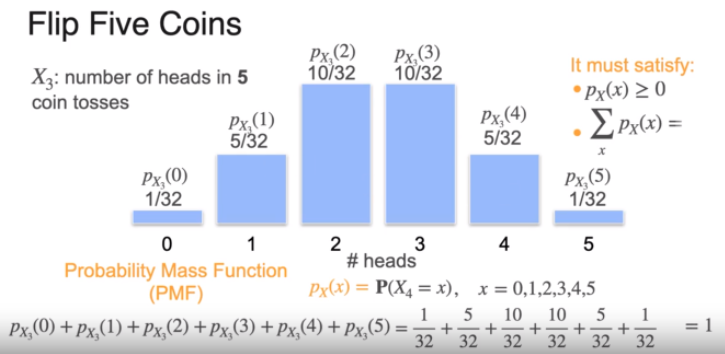
\includegraphics[width=0.85\linewidth]{images/coin_flip.png}
    \caption{PMF – Xác suất số lần xuất hiện mặt ngửa khi tung 5 đồng xu}
\end{figure}

Công thức trên chính là Hàm khối lượng xác suất (Probability Mass Function) viết tắt là PDF giúp mình xem xét cách phân phối xác suất giữa tất cả các biến.  Ví  cho thấy  xác suất xảy ra từng số lượng mặt ngửa khi tung 5 đồng xu, ký hiệu là $X_3$ với tổng cả xác suất luôn bằng 1.
\[
\sum_{x=0}^{5} p_X(x) = 1
\]


\textbf{Quan sát:} Các biến $X_1, X_2, X_3, X_4$ – đại diện cho số lần xuất hiện mặt ngửa khi tung $n$ đồng xu – đều có phân phối xác suất tương tự nhau (e.g.  chia cho 32). Liệu có một mô hình thống nhất để biểu diễn các biến này?

\begin{center}
    \textbf{→ Câu trả lời là: Phân phối nhị thức (Binomial Distribution)}
\end{center}

\vspace{1em}


\section{Phần 3: Probability Distribution (From Discrete to Continuous)}
\subsection{PMF (Probability Mass Function)}
\textbf{Phân phối nhị thức là gì?} \\

Phân phối nhị thức mô tả xác suất xảy ra đúng $k$ lần thành công sau $n$ lần lặp lại một phép thử mà:
\begin{itemize}
    \item Mỗi lần thử chỉ có hai kết quả: \textbf{thành công (1)} hoặc \textbf{thất bại (0)}.
    \item Xác suất thành công ở mỗi lần là như nhau, ký hiệu là $p$.
\end{itemize}

Ví dụ: tung đồng xu nhiều lần, mỗi lần chỉ có mặt ngửa hoặc sấp.

\vspace{1em}

\textbf{Giải thích trực quan hệ số nhị thức:}

\begin{figure}[H]
    \centering
    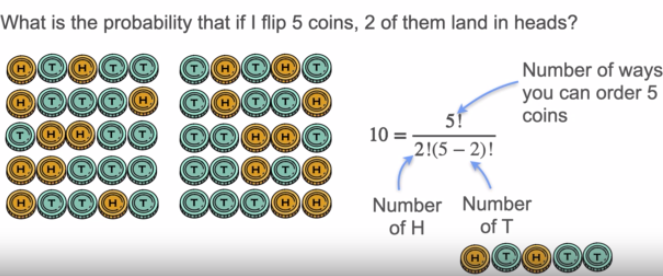
\includegraphics[width=0.9\linewidth]{images/binomial_coefficient.png}
    \caption{Hệ số nhị thức – số cách chọn 2 mặt ngửa trong 5 lần tung đồng xu}
\end{figure}

Trong ví dụ này, ta xét xác suất có đúng 2 mặt ngửa khi tung 5 đồng xu.

\begin{itemize}
    \item $5!$: số cách sắp xếp 5 đồng xu.
    \item Nhưng khi tung 5 đồng xu đó có trùng lặp: 2 mặt ngửa giống nhau và 3 mặt sấp giống nhau. Do ta chỉ quan tâm đến trường hợp có đúng 2 ngửa và 3 sấp, nên cần loại bỏ các hoán vị giống nhau bằng cách chia cho $2! \cdot 3!$.
    \item Kết quả:
    \[
    \binom{5}{2} = \frac{5!}{2!(5-2)!} = 10
    \]
\end{itemize}

→ Có 10 cách để xuất hiện đúng 2 mặt ngửa trong 5 lần tung.

\vspace{1em}

\textbf{Công thức phân phối nhị thức:}
\[
P(X = k) = \binom{n}{k} p^k (1 - p)^{n - k}
\]

Trong đó:
\begin{itemize}
    \item $n$: số lần thử (ví dụ: 5 lần tung đồng xu)
    \item $k$: số lần thành công mong muốn (ví dụ: 2 mặt ngửa)
    \item $p$: xác suất thành công mỗi lần thử (ví dụ: $p = 0.5$ nếu đồng xu công bằng)
    \item $\binom{n}{k}$: hệ số nhị thức – số cách chọn $k$ lần thành công trong $n$ lần thử
\end{itemize}

\vspace{1em}

\begin{summarybox}
    \textbf{Ghi nhớ nhanh:} 
    \begin{itemize}
        \item Biến ngẫu nhiên rời rạc nhận các giá trị rời rạc, ví dụ như số mặt ngửa.
        \item Phân phối nhị thức mô tả xác suất xảy ra đúng $k$ lần thành công trong $n$ phép thử có hai khả năng xảy ra.
        \item Các giá trị rời rạc được mô tả bằng \textbf{Hàm khối xác suất (PMF)}.
    \end{itemize}
\end{summarybox}

\subsection{PDF (Probability Density Function)}
Trong phần trước, chúng ta đã tìm hiểu cách mô tả xác suất của biến ngẫu nhiên rời rạc thông qua hàm khối xác suất (PMF),  mỗi giá trị rời rạc như $0, 1, 2,...$ đều gắn với một xác suất cụ thể. \\ 

Tuy nhiên, trong thực tế, có rất nhiều hiện tượng không thể gắn với giá trị rời rạc mà thay vào đó là \textbf{một khoảng giá trị liên tục} — ví dụ như thời gian, chiều cao, tốc độ,... Khi đó, chúng ta cần một công cụ mới để mô tả xác suất: \textbf{Hàm mật độ xác suất (Probability Density Function - PDF)}. \\

\noindent \textbf{Hiểu Từ Phân phối Rời Rạc đến Liên Tục} \\ 
Trong phân phối rời rạc, tổng xác suất của tất cả kết quả luôn bằng 1. Nhưng hãy tưởng tượng nếu ta có \textbf{rất nhiều kết quả} (thậm chí vô hạn), thì xác suất tại từng điểm riêng lẻ sẽ dần tiến đến . Ví dụ: nếu có 1000 kết quả, thì mỗi kết quả chỉ có xác suất là $1/1000$. \\

 Vậy nếu xác suất của mọi kết quả đều bằng 0 thì ta tính sai ở đâu ? Ta không sai – mà là vì loại phân phối này \textbf{khác về bản chất}. Nó không phải là rời rạc, mà là \textbf{liên tục}. Do vậy, cách tiếp cận cũ (PMF) sẽ không còn hiệu quả.
0
\vspace{1em}

Thay vì hỏi: “Cuộc gọi kéo dài đúng 2 phút có xác suất bao nhiêu?”, hãy đặt câu hỏi theo khoảng: “Cuộc gọi kéo dài \textbf{từ 2 đến 3 phút} thì sao?”

\begin{itemize}
    \item Ban đầu: ta chia các khoảng thành [2, 3], [3, 4]…
    \item Sau đó: chia nhỏ hơn nữa thành [2, 2.5], [2.5, 3]…
    \item Rồi lại tiếp tục chia nhỏ vô hạn như [2, 2.1], [2.1, 2.2]...
\end{itemize}

Khi ta chia nhỏ đến mức vô hạn, ta bắt đầu thấy được một đường cong — hình dung mỗi cột xác suất rất nhỏ tạo thành một đồ thị mượt. Đây chính là lúc chúng ta chuyển sang \textbf{Phân phối liên tục (Continuous Distribution)}. 

\newpage

\textbf{Minh họa: Từ PMF đến PDF} cho thấy cách xác suất “chuyển hóa” từ các cột rời rạc sang 1 đường cong liên tục:
\begin{figure}[H]
    \centering % Căn giữa toàn bộ figure
    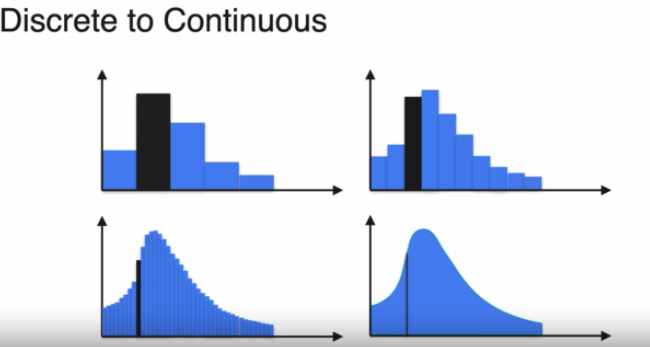
\includegraphics[width=0.6\textwidth]{images/dis2con.png} % Điều chỉnh width cho phù hợp, ví dụ 80% chiều rộng văn bản
    \caption*{\textbf{Phân phối rời rạc (PMF)}} % Nếu chú thích này là của hình ảnh, không phải của subfigure
    \caption{Từ phân phối xác suất rời rạc đến liên tục} 
\end{figure}

\vspace{1em}

\textbf{Cách tính xác suất từ PDF:} \\

Hàm mật độ xác suất (Probability Density Function – viết tắt là \textbf{PDF}) được ký hiệu là $f_X(x)$. Đây là hàm mô tả \textbf{tốc độ tích lũy xác suất quanh mỗi điểm} trong không gian liên tục. PDF chỉ áp dụng cho \textbf{biến ngẫu nhiên liên tục}, và thỏa các điều kiện: \\

\begin{itemize}
    \item $f_X(x) \geq 0$ với mọi $x$
    \item Diện tích toàn bộ dưới đường cong của $f_X(x)$ bằng 1:
    \[
    \int_{-\infty}^{\infty} f_X(x) \, dx = 1
    \]
\end{itemize}

Ta không thể hỏi “xác suất để $X = a$”, vì:
\[
P(X = a) = 0
\]

Thay vào đó, ta tính xác suất để $X$ nằm trong một \textbf{khoảng giá trị} $(a, b)$ bằng cách lấy \textbf{diện tích dưới đường cong} $f_X(x)$ từ $a$ đến $b$:

\[
P(a < X < b) = \int_a^b f_X(x) \, dx
\]

\vspace{1em}	

\begin{summarybox}
    \textbf{Ghi nhớ nhanh:} 
    \begin{itemize}
        \item PMF: Dùng cho biến rời rạc. Xác suất tại từng điểm rời rạc. Tổng các xác suất = 1.
        \item PDF: Dùng cho biến liên tục. Xác suất trong một khoảng → tính bằng \textbf{diện tích dưới đường cong}.
        \item $P(X = a) = 0$ là xác suất ở từng điểm băng 0 với biến liên tục.
        \item PDF không cho ta “xác suất” mà là “mật độ” — tức là mức độ tích lũy xác suất quanh một điểm.
        \item Tính xác suất bằng tích phân: $\displaystyle P(a < X < b) = \int_a^b f_X(x)\, dx$
    \end{itemize}
\end{summarybox}

\subsection{CMF (Cumulative Probability Function)}

\textbf{Động lực xuất hiện CDF:} \\

Ở phần trước, ta biết rằng khi làm việc với PDF (hàm mật độ xác suất), ta phải tính tích phân — tức là \textbf{tính diện tích dưới đường cong} — để tìm xác suất trong một khoảng. Nhưng điều này không phải lúc nào cũng thuận tiện, nhất là khi ta cần biết xác suất tích lũy từ điểm bắt đầu đến một giá trị cụ thể.

Đó là lý do vì sao ta cần đến \textbf{Hàm phân phối tích lũy – Cumulative Distribution Function (viết tắt là CDF hoặc CMF)}.

\vspace{1em}

\textbf{CDF là gì?} \\

CDF cho biết \textbf{xác suất tích lũy} mà biến ngẫu nhiên $X$ nhỏ hơn hoặc bằng một giá trị cụ thể $x$:

\[
F_X(x) = P(X \leq x)
\]

Tức là CDF sẽ “cộng dồn” tất cả xác suất từ $-\infty$ đến $x$. Đây là \textbf{tổng diện tích} dưới đường cong PDF từ trái qua phải đến điểm $x$.

\vspace{1em}

\textbf{Khác biệt giữa PDF và CDF:}
\begin{itemize}
    \item \textbf{PDF} cho biết xác suất trong một khoảng cụ thể (i.e. là chiều cao tại 1 khoảng)
    \item \textbf{CDF} cho biết tổng xác suất từ điểm bắt đầu cho đến một giá trị nhất định (i.e. diện tích tích lũy)
\end{itemize}

\textbf{Ví dụ trực quan:}

\begin{figure}[H]
    \centering
    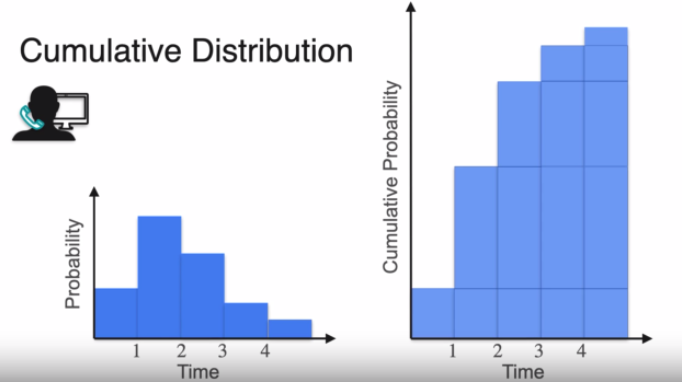
\includegraphics[width=0.8\linewidth]{images/pdf2cmf.png}
    \caption{So sánh PDF và CDF – tích lũy xác suất từ 0 đến 1, rồi 0 đến 2,...}
\end{figure}

\vspace{0.5em}

\textbf{Tính chất của CDF:}
\begin{itemize}
    \item $F_X(x)$ (tổng xác suất của X) luôn nằm trong khoảng $[0, 1]$
    \item Luôn \textbf{tăng dần} vì xác suất tích lũy không thể âm
    \item Càng về bên phải, CDF càng tiến gần đến 1
\end{itemize}

\vspace{1em}

\textbf{Ví dụ cho PDF liên tục}

\begin{figure}[H]
    \centering
    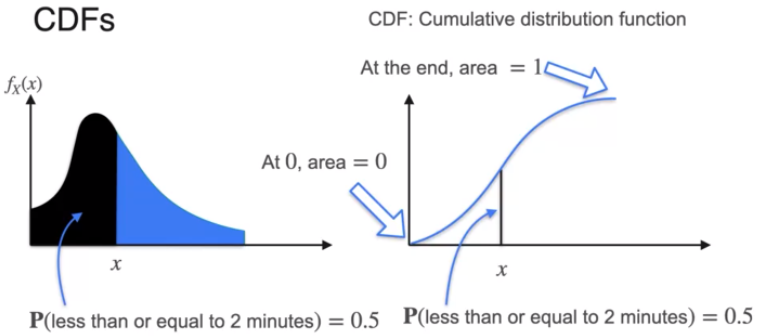
\includegraphics[width=0.8\linewidth]{images/pdf2cmf2.png}
    \caption{CDF khi PDF liên tục trong 1 khoảng}
\end{figure}

\vspace{1em}

\begin{summarybox}
    \textbf{Ghi nhớ nhanh:}
    \begin{itemize}
        \item PDF: Cho biết mật độ xác suất tại một điểm. Phải dùng tích phân để tính xác suất theo khoảng.
        \item CDF: Cho biết tổng xác suất từ đầu đến điểm $x$, ký hiệu là $F_X(x) = P(X \leq x)$.
        \item CDF luôn nằm trong khoảng $[0, 1]$ và không bao giờ giảm.
        \item CDF giúp ta \textbf{tránh tính tích phân lặp đi lặp lại} — ta chỉ cần lấy hiệu giữa $F_X(b) - F_X(a)$ để biết xác suất $P(a < X < b)$.
    \end{itemize}
\end{summarybox}

\section{Phần 4: Mean/Expected Value, Variance, Standard Deviation và ứng dụng của chúng}
\subsection{Expected Value}

\textbf{Giá trị kỳ vọng là gì?} \\
Trong thống kê, \textbf{Mean (giá trị trung bình)} là trung bình cộng của một tập hợp dữ liệu — ví dụ như điểm số trung bình của sinh viên hoặc thời gian chờ xe buýt. Khi làm việc với biến ngẫu nhiên, giá trị trung bình này được gọi là \textbf{Expected Value (Giá trị kỳ vọng)}. Nói cách khác:
\begin{center}
    \textit{Expected Value chính là trung bình có trọng số của tất cả các kết quả có thể xảy ra, dựa trên xác suất xảy ra của chúng.}
\end{center}

\begin{figure}[H]
    \centering % Căn giữa toàn bộ figure
    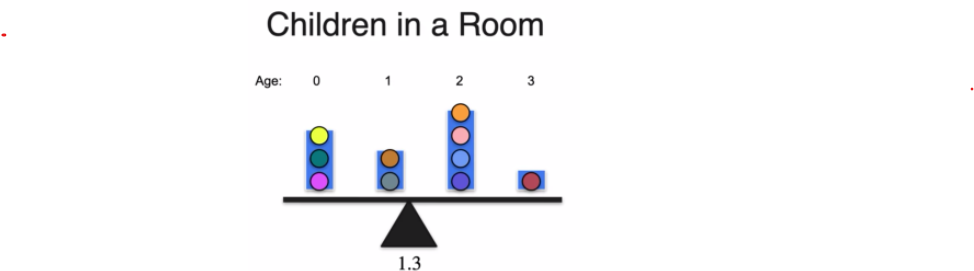
\includegraphics[width=1.2\linewidth]{images/expected_value_equilibrium.png}
    \caption{Ví dụ: Tính giá trị kỳ vọng tuổi của trẻ em trong phòng}
\end{figure}



Giả sử trong một lớp học có 10 em nhỏ với độ tuổi lần lượt là: 0, 0, 0, 1, 1, 2, 2, 2, 2, 3.

Khi đó:
\[
\mathbb{E}[X] = \frac{0 + 0 + 0 + 1 + 1 + 2 + 2 + 2 + 2 + 3}{10} = \frac{13}{10} = 1.3
\]

Tức là tuổi trung bình (expected value) là 1.3.

Ta có thể xem đây là một \textbf{trung bình có trọng số}, trong đó:
\begin{itemize}
    \item Có 3 em 0 tuổi → $P(X=0) = \frac{3}{10}$
    \item Có 2 em 1 tuổi → $P(X=1) = \frac{2}{10}$
    \item Có 4 em 2 tuổi → $P(X=2) = \frac{4}{10}$
    \item Có 1 em 3 tuổi → $P(X=3) = \frac{1}{10}$
\end{itemize}

Từ đó:
\[
\mathbb{E}[X] = 0 \cdot \frac{3}{10} + 1 \cdot \frac{2}{10} + 2 \cdot \frac{4}{10} + 3 \cdot \frac{1}{10} = 1.3
\]

\vspace{1em}

\textbf{Ví dụ thực tế:}
\begin{itemize}
    \item \textbf{Ví dụ 1 – Đặt cược \$5 vào mặt ngửa:} Nếu bạn đặt cược \$5 vào mặt ngửa, xác suất thắng là 0.5 → giá trị kỳ vọng sẽ quyết định bạn nên cược bao nhiêu để không lỗ về lâu dài.
    
    \item \textbf{Ví dụ 2 – Tung 3 đồng xu:} Mỗi mặt ngửa bạn được $1 →$ số tiền trung bình mong đợi sau 3 lần tung là:
    \[
    \mathbb{E}[X] = 0 \cdot \frac{1}{8} + 1 \cdot \frac{3}{8} + 2 \cdot \frac{3}{8} + 3 \cdot \frac{1}{8} = 1.5
    \]
\end{itemize}

\vspace{1em}

\textbf{Vì giá trị kì vọng là trung bình trọng số của phân phối xác suất, ta có thể thấy:}
\begin{itemize}
    \item Với \textbf{biến rời rạc}: giá trị kỳ vọng là điểm cân bằng của \textbf{PMF}
    \item Với \textbf{biến liên tục}: giá trị kỳ vọng là điểm cân bằng của \textbf{PDF}, tính bằng tích phân:
    \[
    \mathbb{E}[X] = \int_{-\infty}^{\infty} x \cdot f_X(x) \, dx
    \]
\end{itemize}

\vspace{1em}

\textbf{Ví dụ liên tục:} Bạn thu thập thời gian chờ xe buýt suốt nhiều năm và nó có phân phối đều (uniform) từ 0 đến 60 phút. Khi đó, trung bình luôn ở chính giữa:
\begin{figure}[H]
    \centering % Căn giữa toàn bộ figure
    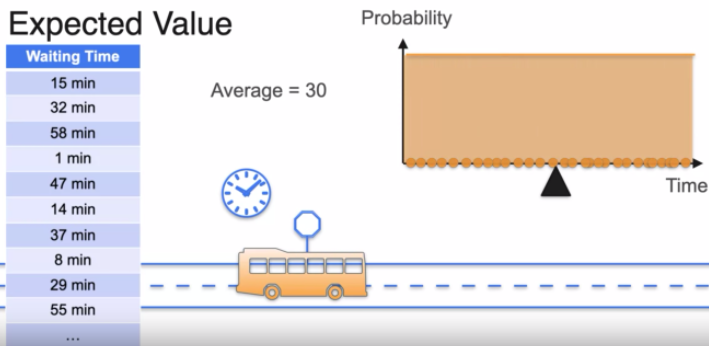
\includegraphics[width=0.7\linewidth]{images/equalDistribution.png}
    \caption{Ví dụ Mean trong phân phối đồng đều}
\end{figure}
\[
\mathbb{E}[X] = \frac{a + b}{2} = \frac{0 + 60}{2} = 30
\]


\vspace{1em}

\textbf{Hiểu nhầm phổ biến:}

Nhiều người cho rằng Expected Value là điểm ở giữa biểu đồ  nhưng nó không phải lúc nào cũng đúng. Nếu dữ liệu bị lệch do một giá trị ngoài lề (outlier như kết quả có khả năng xảy ra cao hơn mọi kết quả khác, điểm của 1 học sinh giỏi trong 1 lớp kém  kéo điểm trung bình của cả lớp lên), điểm cân bằng sẽ bị kéo lệch. Trong khi đó, giá trị ở giữa thật sự là \textbf{Median} — ta sẽ tìm hiểu ở phần tiếp theo.

\vspace{1em}

\begin{summarybox}
    \textbf{Ghi nhớ nhanh:}
    \begin{itemize}
        \item Expected Value là giá trị trung bình mong đợi của một biến ngẫu nhiên.
        \item Với biến rời rạc: $\mathbb{E}[X] = \sum x \cdot P(X = x)$
        \item Với biến liên tục: $\mathbb{E}[X] = \int x \cdot f_X(x) \, dx$
        \item Expected Value là điểm cân bằng của phân phối xác suất.
        \item Giá trị này có thể bị ảnh hưởng mạnh bởi outlier (giá trị dị biệt).
    \end{itemize}
\end{summarybox}

\subsection{Median}

\textbf{Khi Mean có thể đánh lừa:}

Mặc dù Mean (giá trị trung bình) giúp mô tả xu hướng trung tâm của dữ liệu, nhưng trong một số trường hợp, nó có thể không phản ánh chính xác "giá trị điển hình" — đặc biệt là khi xuất hiện \textbf{Outlier (giá trị ngoại lệ)}. Ví dụ như khi lương của 1 người cực kì cao làm nghiên cán cân mức lương trung bình của tất cả học sinh tốt nghiệp ở trường đại học cao hơn. Đây là khi xác suất có thể lừa dối. 

\begin{figure}[H]
    \centering
    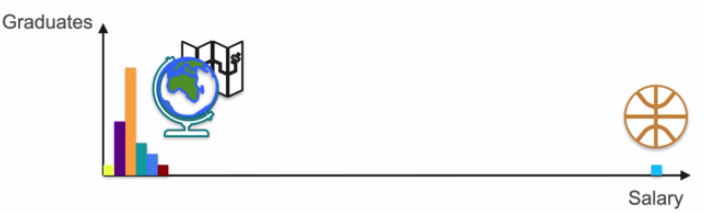
\includegraphics[width=0.9\linewidth]{images/mean_salary_outlier_example.png}
    \caption{Giá trị trung bình bị ảnh hưởng mạnh bởi một phần tử quá lớn}
\end{figure}

\textbf{Outlier} làm lệch toàn bộ dữ liệu và khiến Mean trở nên sai lệch.

\vspace{1em}

\textbf{Lúc này, Median là lựa chọn tốt hơn:}
Sắp xếp toàn bộ dữ liệu theo thứ tự tăng dần, rồi chọn ra \textbf{giá trị ở giữa}. Đây là \textbf{Median – trung vị}, đại diện cho giá trị "ở giữa" tập dữ liệu (nếu tập dữ liệu chẵn sẽ lấy trung bình của 2 trung vị). Trong ví dụ trên, mình sắp xếp từng người với mức lương từ thâp đến cao rồi chọn trung điểm làm Median.

\begin{figure}[H]
    \centering
    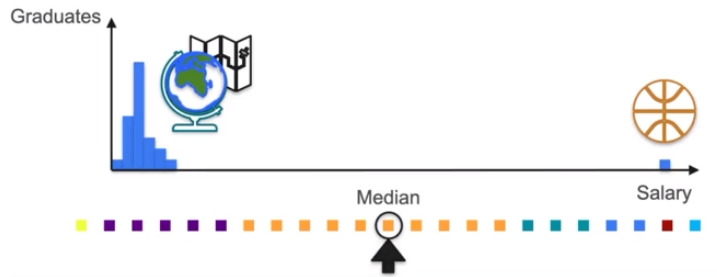
\includegraphics[width=0.85\linewidth]{images/median_salary_outlier_example.png}
    \caption{Lấy Median từ tập dữ liệu sau khi sắp xếp}
\end{figure}

\textbf{Định nghĩa:} Median là \textbf{giá trị trung vị} trong một tập dữ liệu đã được sắp xếp.\\

\textbf{Cách tính Median:}
\begin{itemize}
    \item Với tập dữ liệu lẻ (ví dụ có 5 phần tử): Median là giá trị ở vị trí $\frac{N+1}{2}$
    \item Với tập dữ liệu chẵn (ví dụ có 6 phần tử): Median là trung bình của 2 phần tử ở giữa vì chúng đều là trung điểm:
    \[
    \text{Median} = \frac{S\left( \frac{N}{2} \right) + S\left( \frac{N}{2} + 1 \right)}{2}
    \]
\end{itemize}

\vspace{1em}

\textbf{Ví dụ thêm:}

Xét tập dữ liệu: \texttt{1, 2, 3, 4, 100}

\begin{itemize}
    \item \textbf{Mean:} $(1 + 2 + 3 + 4 + 100)/5 = 22$ → bị ảnh hưởng mạnh bởi outlier.
    \item \textbf{Median:} giá trị ở giữa là \texttt{3} → thể hiện giá trị điển hình hơn.
\end{itemize}

\vspace{1em}

\textbf{Mode – Giá trị phổ biến nhất:}

Ngoài Mean và Median, còn một khái niệm khác gọi là \textbf{Mode} – là \textbf{giá trị xuất hiện nhiều nhất} trong tập dữ liệu.

\begin{figure}[H]
    \centering
    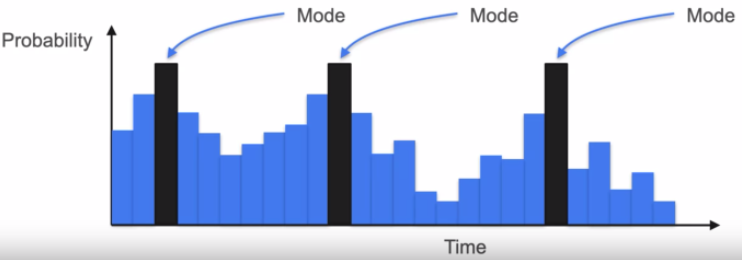
\includegraphics[width=0.6\linewidth]{images/mode_multimodal.png}
    \caption{Một phân phối có thể có nhiều Mode (đa đỉnh)}
\end{figure}

\begin{itemize}
    \item Mode phù hợp để mô tả trung tâm dữ liệu khi các giá trị rơi vào các cụm rõ rệt.
    \item Trong phân phối nhị thức hoặc các trường hợp rời rạc khác, Mode là giá trị có xác suất cao nhất.
\end{itemize}

\vspace{1em}

\textbf{Tổng kết sự khác nhau giữa Mean – Median – Mode:}

\begin{figure}[H]
    \centering
    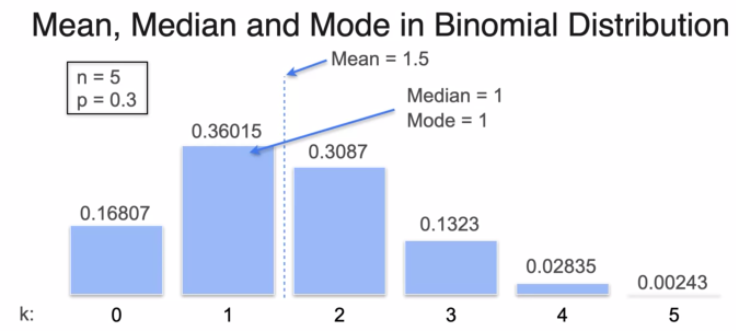
\includegraphics[width=0.8\linewidth]{images/mean_median_mode_comparison.png}
    \caption{So sánh Mean, Median và Mode trong các trường hợp phân phối khác nhau}
\end{figure}

\begin{itemize}
    \item \textbf{Mean:} điểm cân bằng trung tâm – bị ảnh hưởng bởi outlier.
    \item \textbf{Median:} giá trị ở giữa – phù hợp khi dữ liệu lệch (skewed).
    \item \textbf{Mode:} giá trị xuất hiện phổ biến nhất – phù hợp khi có nhiều cụm dữ liệu.
    \item \textbf{Trong Uniform Distribution} vì dữ liệu và giá trị phân phối đồng đều nên Mean, Median sẽ ở cùng 1 điểm.    \\ 
\end{itemize}

\section{Phần 5 Mở rộng: Giá trị kỳ vọng của 1 hàm số và Tổng của kỳ vọng}
Đây là phần quan trọng để ta có thể hiểu được công thức của Variance. 

\subsection{Giá trị kỳ vọng của một Hàm số (Expected Value of a Function)}
\textbf{Khi nào cần kỳ vọng của một hàm số?}  
Sau khi hiểu cách tính kỳ vọng (Expected Value) của biến ngẫu nhiên $X$, câu hỏi đặt ra là:  
\textit{Điều gì sẽ xảy ra nếu ta không chỉ quan tâm đến giá trị $X$, mà quan tâm đến một hàm của $X$ như $X^2$, $X^3$, hay $g(X)$ bất kỳ?}

\vspace{0.5em}
\textbf{Ý tưởng trực quan:}

\begin{itemize}
    \item Với mỗi giá trị $x_i$ xảy ra với xác suất $p(x_i)$, kỳ vọng $\mathbb{E}[X]$ được tính bằng tổng $x_i \cdot p(x_i)$.
    \item Nếu bạn muốn tính kỳ vọng của $X^2$, chỉ cần thay thế $x_i$ bằng $x_i^2$, tức là $\mathbb{E}[X^2] = \sum x_i^2 \cdot p(x_i)$.
    \item Tổng quát: Nếu bạn muốn tính kỳ vọng của một hàm $g(X)$, thì:
    \[
    \mathbb{E}[g(X)] = \sum g(x_i) \cdot p(x_i)
    \]
\end{itemize}

\begin{figure}[H]
    \centering
    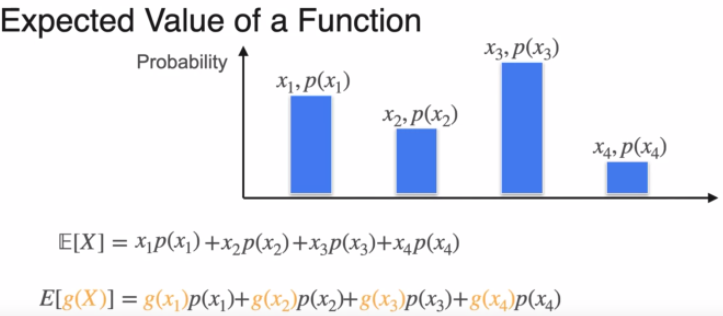
\includegraphics[width=0.85\linewidth]{images/expected_value_function.png}
    \caption{So sánh công thức kỳ vọng và công thức kỳ vọng của một hàm $g(X)$}
\end{figure}

\vspace{0.5em}

\textbf{Ví dụ 1: Kỳ vọng của $X^2$ – Trò chơi xúc xắc}
\begin{itemize}
    \item Tung một viên xúc xắc, nếu ra mặt $x$, bạn nhận phần thưởng là $x^2$ đô.
    \item Hỏi: Bạn nên trả để chơi trò này? 
\end{itemize}

Tính kỳ vọng:
\[
\mathbb{E}[X^2] = \frac{1^2 + 2^2 + 3^2 + 4^2 + 5^2 + 6^2}{6} = \frac{91}{6} \approx 15.17
\]

→ Trung bình bạn nhận được khoảng 15.17 đô → không nên trả nhiều hơn số tiền này để chơi. \\ 

\vspace{0.5em}

\textbf{Ví dụ 2: Kết hợp hàm tuyến tính – $g(x) = 2x - 5$}

\begin{itemize}
    \item Tung xúc xắc và nhận phần thưởng gấp đôi giá trị ($2x$), nhưng phải trả phí 5 đô để tham gia.
    \item Lợi nhuận thực sự mỗi lượt là $g(x) = 2x - 5$
\end{itemize}

\begin{figure}[H]
    \centering
    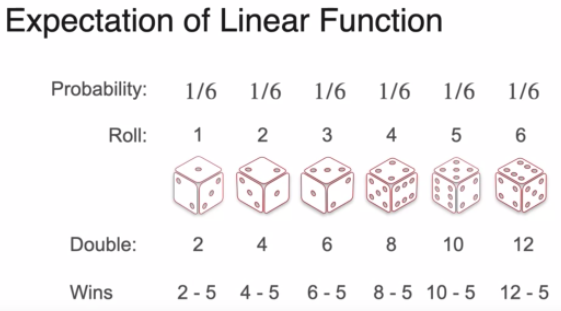
\includegraphics[width=0.7\linewidth]{images/dice_game_net_reward.png}
    \caption{Giá trị lợi nhuận: $g(x) = 2x - 5$}
\end{figure}

Tính kỳ vọng:
\[
\mathbb{E}[g(X)] = \mathbb{E}[2X - 5] = 2 \cdot \mathbb{E}[X] - 5
\]
\[
\text{Vì } \mathbb{E}[X] = \frac{1 + 2 + 3 + 4 + 5 + 6}{6} = 3.5
\Rightarrow \mathbb{E}[g(X)] = 2 \cdot 3.5 - 5 = 2
\]

→ Trung bình bạn lời được 2 đô mỗi lượt.

\vspace{0.5em}

\textbf{Tính chất quan trọng: Expected Value là toán tử tuyến tính}

\[
\mathbb{E}[aX + b] = a \cdot \mathbb{E}[X] + b
\]
\[
\mathbb{E}[g_1(X) + g_2(X)] = \mathbb{E}[g_1(X)] + \mathbb{E}[g_2(X)]
\]

\textit{Dù hàm $g(x)$ là tuyến tính hay không, công thức vẫn áp dụng được.}

\vspace{1em}


\begin{summarybox}
	\textbf{Ghi nhớ nhanh:}
	\begin{itemize}
	    \item Chỉ cần thay $x$ bằng $g(x)$ trong công thức kỳ vọng.
	    \item Expected Value có tính tuyến tính: $\mathbb{E}[aX + b] = a \cdot \mathbb{E}[X] + b$.
	    \item $\mathbb{E}[\text{const}] = \text{const}$.
	    \item Có thể dùng để tính các đại lượng như $\mathbb{E}[X^2]$, $\mathbb{E}[|X|]$, $\mathbb{E}[\sqrt{X}]$, v.v.
	\end{itemize}
\end{summarybox}

\subsection{Tổng kỳ vọng – Sum of Expectations}

\textbf{Ví dụ 1:} Tung một đồng xu và một xúc xắc:
\begin{itemize}
    \item Nếu ra ngửa: thắng 1 đô
    \item Sau đó tung xúc xắc và nhận đúng số tiền bằng mặt xúc xắc
\end{itemize}

\begin{figure}[H]
    \centering
    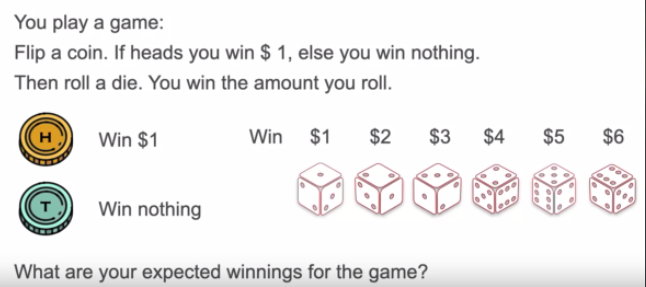
\includegraphics[width=0.8\linewidth]{images/coin_dice_expectation.png}
    \caption{Tổng kỳ vọng từ 2 hành động độc lập}
\end{figure}

\[
\mathbb{E}[X] = \mathbb{E}[X_{\text{coin}}] + \mathbb{E}[X_{\text{dice}}] = 0.5 + 3.5 = 4
\]

\textbf{Kết luận:} 
\[
\mathbb{E}[X + Y] = \mathbb{E}[X] + \mathbb{E}[Y] 
\] \\ \\


 
\textbf{Ví dụ 2: Bao nhiêu người được gán đúng tên?} \\ 
Bạn có 1 túi chứa các tên ngẫu nhiên của 8 tỷ người. Nếu bạn rút ngẫu nhiên một tờ từ túi và mỗi người chỉ nhận đúng 1 tên, trung bình có bao nhiêu người chọn ra đúng tên của mình ?

\vspace{0.5em}

\textbf{Theo trực giác, bạn sẽ nghĩ là xác suất rất thấp nhưng sự thật sẽ có ít nhất 1 người} được chọn đúng tên, vì xác suất là 1/8 tỷ. Để hiểu rõ hơn, mình sẽ lấy ví dụ trực quan với 3 người: Aisha, Beto và Cameron thay vì 8 tỷ người.

\vspace{1em}

Có tất cả $3! = 6$ hoán vị để phân phối tên cho 3 người. (i.e. các trường hợp có thể xảy ra khi lấy lần lượt từng tên ra khỏi túi).

\begin{figure}[H]
    \centering
    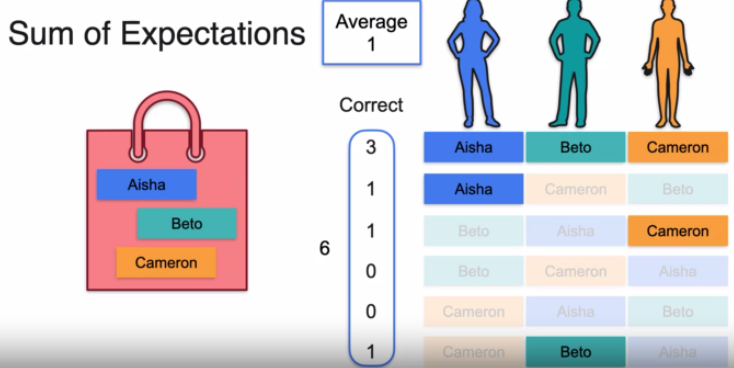
\includegraphics[width=0.9\linewidth]{images/sum_expectation_names.png}
    \caption{Số lần gán đúng tên trong từng hoán vị}
\end{figure}

Tổng số lượt đúng: $3 + 1 + 1 + 0 + 0 + 1 = 6$  
Trung bình sau 6 hoán vị: $6 / 6 = 1$

→ Với 3 người, số người nhận đúng tên trung bình là 1. Vậy còn 8 tỷ người?

\vspace{1em}

\textbf{Sử dụng Sum of Expectations để tổng quát:}

Gọi biến ngẫu nhiên $M_i$ là 1 nếu người thứ $i$ nhận đúng tên mình, và $0$ nếu sai.

Xác suất để người $i$ nhận đúng tên: $\mathbb{P}(M_i = 1) = \frac{1}{n}$

\[
\mathbb{E}[M_i] = 1 \cdot \frac{1}{n} + 0 \cdot \left(1 - \frac{1}{n}\right) = \frac{1}{n}
\]

Tổng số người được gán đúng tên là:
\[
M = \sum_{i=1}^n M_i
\Rightarrow \mathbb{E}[M] = \sum_{i=1}^n \mathbb{E}[M_i] = n \cdot \frac{1}{n} = 1
\]
Đơn giản vì tổng của 8 tỷ lần 1/8 tỷ = 1
→ \textbf{Không phụ thuộc vào $n$, kỳ vọng luôn bằng 1!} 

\vspace{0.5em}

\begin{summarybox}
    \textbf{Ghi nhớ nhanh:}
    \begin{itemize}
        \item Dù có 5, 500 hay 8 tỷ người, số người trung bình được gán đúng tên là 1.
        \item Đây là minh chứng trực quan cho tính chất \textbf{cộng tuyến tính của kỳ vọng}:
        \[
        \mathbb{E}[X_1 + X_2 + \ldots + X_n] = \mathbb{E}[X_1] + \mathbb{E}[X_2] + \ldots + \mathbb{E}[X_n]
        \]
        \item Tính chất này đúng kể cả khi các biến không độc lập, thường được ứng dụng trong xác suất tổ hợp.
    \end{itemize}
\end{summarybox}

\section{Phần 6: Variance – Phương sai}
\subsection{Động lực: Để miêu tả dữ liệu, kỳ vọng thôi là chưa đủ}
Kỳ vọng rất hữu ích trong việc tóm tắt phân phối. Tuy nhiên, kỳ vọng không phản ánh đầy đủ toàn bộ đặc trưng của phân phối.  Ví dụ, ta có thể có hai trò chơi (hay hai biến ngẫu nhiên) có \textbf{cùng kỳ vọng bằng 0}, nhưng một trò chỉ dao động từ $-1$ đến $+1$, còn trò kia dao động từ $-100$ đến $+100$. \\

Cả hai trò đều "cân bằng" tại giá trị 0, nhưng rõ ràng \textbf{độ biến động (spread)} của chúng là rất khác nhau.   Sự khác biệt này được đo bởi một khái niệm mới: \textbf{Phương sai (variance)}.

\vspace{1em}

\subsection{Ví dụ: So sánh hai trò chơi}

\textbf{Game 1:} Gieo đồng xu, nếu ra mặt ngửa thì thắng \$1, nếu ra mặt sấp thì thua \$1.  
$\Rightarrow$ Xác suất 50–50, kỳ vọng là:
\[
\mathbb{E}[X_1] = 0.5 \cdot (-1) + 0.5 \cdot 1 = 0
\]

\textbf{Game 2:} Gieo đồng xu, nếu ra mặt ngửa thì thắng \$100, nếu ra mặt sấp thì thua \$100.  
Kỳ vọng vẫn là:
\[
\mathbb{E}[X_2] = 0.5 \cdot (-100) + 0.5 \cdot 100 = 0
\]

\textit{Kết luận:} Hai trò chơi có cùng kỳ vọng, nhưng trò thứ hai có mức độ rủi ro cao hơn rõ ràng.

\vspace{1em}

\subsection{Ta cần đo độ “lan rộng” của phân phối}

Giả sử ta đo \textbf{sai lệch (deviation)} của từng kết quả so với kỳ vọng.  
Với Game 1: ta có các sai lệch là $+1$ và $-1$  
Với Game 2: ta có các sai lệch là $+100$ và $-100$.

Nếu ta lấy trung bình các sai lệch này:
\[
\frac{1 + (-1)}{2} = 0 \quad \text{(luôn luôn bằng 0)}
\]

Điều này không hữu ích. Các sai lệch âm và dương triệt tiêu nhau.  
Một hướng khác là dùng \textbf{giá trị tuyệt đối} (absolute deviation), nhưng phương pháp này không tiện về mặt toán học.

\textbf{Giải pháp tối ưu:} Ta dùng \textbf{bình phương sai lệch} – tức là lấy $(x - \mu)^2$, nhờ đó mọi giá trị đều dương và dễ xử lý toán học.

\vspace{1em}

\subsection{Rút công gọn thức phương sai từ kỳ vọng}

Công thức định nghĩa phương sai của một biến ngẫu nhiên $X$ với kỳ vọng $\mu = \mathbb{E}[X]$ là:
\[
\text{Var}(X) = \mathbb{E}[(X - \mathbb{E}[X])^2]
\]

Ta sẽ chứng minh rằng công thức trên tương đương với:
\[
\text{Var}(X) = \mathbb{E}[X^2] - (\mathbb{E}[X])^2
\]

\textbf{Bước 1: Khai triển bình phương trong kỳ vọng}
\[
\text{Var}(X) = \mathbb{E}\left[(X - \mu)^2\right] = \mathbb{E}\left[X^2 - 2\mu X + \mu^2\right]
\]

\textbf{Bước 2: Tính kỳ vọng từng thành phần} \\
Do tính chất tuyến tính của kỳ vọng:
\[
\mathbb{E}[X^2 - 2\mu X + \mu^2] = \mathbb{E}[X^2] - 2\mu \mathbb{E}[X] + \mathbb{E}[\mu^2]
\]

\textbf{Bước 3: Rút gọn} \\
Vì $\mu = \mathbb{E}[X]$ là hằng số nên:
\[
\mathbb{E}[X^2] - 2\mu \cdot \mu + \mu^2 = \mathbb{E}[X^2] - 2\mu^2 + \mu^2 = \mathbb{E}[X^2] - \mu^2
\]

Do đó:
\[
\text{Var}(X) = \mathbb{E}[X^2] - (\mathbb{E}[X])^2
\]

Kết luận: hai công thức là tương đương và thường trong thực hành, ta sử dụng công thức rút gọn $\mathbb{E}[X^2] - (\mathbb{E}[X])^2$ vì dễ tính toán hơn.


\subsection{Công thức phương sai}

Cho biến ngẫu nhiên $X$ với kỳ vọng $\mu = \mathbb{E}[X]$, phương sai được định nghĩa là:
\[
\text{Var}(X) = \mathbb{E}[X^2] - (\mathbb{E}[X])^2
\]

Các bước để tính phương sai:
\begin{enumerate}
    \item Tính kỳ vọng $\mu$
    \item Tính sai lệch: $(x - \mu)$ cho từng giá trị
    \item Bình phương sai lệch: $(x - \mu)^2$
    \item Lấy kỳ vọng của bình phương sai lệch
\end{enumerate}

Ví dụ:
\begin{itemize}
    \item Game 1: các sai lệch là $+1$ và $-1$, bình phương là $1$ và $1$, trung bình là 1.
    \item Game 2: các sai lệch là $+100$ và $-100$, bình phương là $10{,}000$ và $10{,}000$, trung bình là 10,000.
\end{itemize}

\textbf{Tóm lại:} Game 2 có mức độ biến động cao hơn rất nhiều.

\vspace{1em}

\subsection{Thuộc tính của phương sai}

Một thuộc tính cực kỳ quan trọng của phương sai là:

\[
\text{Var}(aX + b) = a^2 \cdot \text{Var}(X)
\]

\begin{itemize}
    \item Cộng thêm hằng số $b$ không làm thay đổi phương sai.
    \item Nhưng nhân với hằng số $a$ thì làm phương sai tăng theo $a^2$. 
\end{itemize}


\textbf{Ví dụ:}  
\begin{figure}[H]
    \centering
    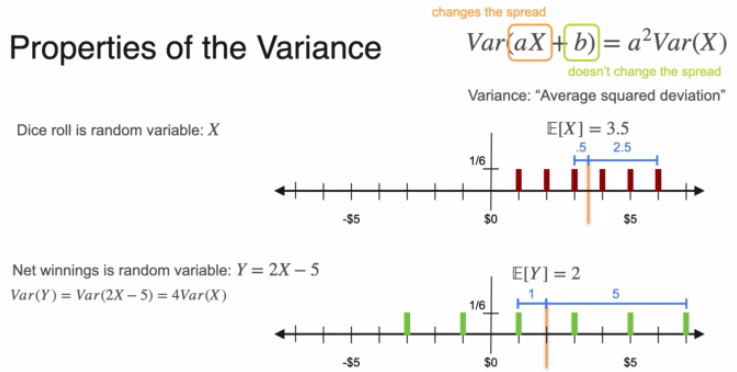
\includegraphics[width=0.8\linewidth]{images/variance_property.png}
    \caption{Tổng kỳ vọng từ 2 hành động độc lập}
\end{figure}
Nếu biến $X$ có phương sai là $2$  
thì biến $Y = 3X + 5$ sẽ có phương sai là $3^2 \cdot 2 = 18$

Điều này rất quan trọng khi bạn biến đổi dữ liệu: nhân dữ liệu với một số sẽ thay đổi mức độ phân tán (spread), còn cộng thì chỉ làm dữ liệu “dời vị trí” chứ không thay đổi phương sai.

\vspace{1em}

\begin{summarybox}
    \textbf{Tóm tắt :}
    \begin{itemize}
        \item Expected value không nói hết phân phối – cần đo độ phân tán.
        \item Variance là kỳ vọng của bình phương sai lệch.
        \item Công thức: $\text{Var}(X) = \mathbb{E}[(X - \mathbb{E}[X])^2] = \mathbb{E}[X^2] - (\mathbb{E}[X])^2$
        \item $\text{Var}(aX + b) = a^2 \cdot \text{Var}(X)$
    \end{itemize}
\end{summarybox}

\newpage 

\section{Phần 7: Standard Deviation}
Phương sai (\textit{variance}) là một cách rất hữu ích để đo mức độ phân tán của một phân phối.  
Tuy nhiên, nó có một nhược điểm nhỏ: \textbf{đơn vị đo không giống với đơn vị dữ liệu gốc}.

Hãy xem xét ví dụ về chiều cao của người:
\begin{itemize}
    \item Chiều cao đo bằng mét ($m$) -  $X$ sẽ dùng $m$
    \item Kỳ vọng (trung bình) cũng có đơn vị là mét - $E[X^2]$ và $E[X]^2$ sẽ dùng $m^2$ vì X là hằng số
    \item Nhưng phương sai lại có đơn vị là mét bình phương ($m^2$) - Var(X) cũng sẽ dùng $m^2$
\end{itemize}

Điều này khiến phương sai trở nên khó trực quan hoá, vì mét vuông thường dùng để đo diện tích chứ không phải chiều cao.

\vspace{0.5em}
\noindent
\textbf{Giải pháp:} Để làm cho đơn vị trở nên “đúng đắn” và dễ hiểu hơn, ta \textbf{lấy căn bậc hai của phương sai}.  
Kết quả nhận được gọi là \textbf{độ lệch chuẩn (standard deviation)}.

\vspace{1em}
\textbf{Định nghĩa:}

\[
\sigma = \sqrt{\text{Var}(X)} = \sqrt{\mathbb{E}[(X - \mu)^2]}
\]

Trong đó:
\begin{itemize}
    \item $\sigma$: độ lệch chuẩn
    \item $\mu$: kỳ vọng của $X$ (tức là $\mathbb{E}[X]$)
    \item $X$: biến ngẫu nhiên
\end{itemize}

\vspace{1em}
\textbf{Ví dụ:}  
Giả sử ta có tập dữ liệu chiều cao của 3 người: 160cm, 170cm, 180cm.
\begin{itemize}
    \item Trung bình: $(160 + 170 + 180)/3 = 170$ cm
    \item Phương sai: $\frac{(160 - 170)^2 + (170 - 170)^2 + (180 - 170)^2}{3} = \frac{100 + 0 + 100}{3} = 66.\bar{6}$ cm$^2$
    \item Độ lệch chuẩn: $\sqrt{66.\bar{6}} \approx 8.16$ cm
\end{itemize}

Như vậy, độ lệch chuẩn giúp ta mô tả độ phân tán của chiều cao với cùng đơn vị là cm – dễ hiểu hơn nhiều so với đơn vị cm$^2$ của phương sai.

\vspace{1em}
\begin{tcolorbox}[colback=yellow!5!white,colframe=yellow!60!black,title=Ghi nhớ]
\textbf{Độ lệch chuẩn là căn bậc hai của phương sai.}  
Nó đo độ phân tán của dữ liệu \textbf{cùng đơn vị} với dữ liệu gốc.
\end{tcolorbox}

\vspace{1em}
\begin{summarybox}
    \textbf{Tóm tắt:}
    \begin{itemize}
        \item Expected value không nói lên hết câu chuyện về phân phối – cần đo độ phân tán.
        \item Công thức: $\text{Var}(X) = \mathbb{E}[(X - \mathbb{E}[X])^2] = \mathbb{E}[X^2] - (\mathbb{E}[X])^2$
        \item Standard deviation: $\sigma = \sqrt{\text{Var}(X)}$ – có cùng đơn vị với $X$
    \end{itemize}
\end{summarybox}


\section{Phần 8: Ứng dụng của Mean, Median, Variance}
\subsection{Ứng dụng của Mean}

Trước khi nói đến ứng dụng, ta cần hiểu rõ sự khác biệt giữa Mean và Expected Value (giá trị kỳ vọng).

\begin{itemize}
    \item \textbf{Mean} là giá trị trung bình thu được từ dữ liệu thực tế mà mình đa thu được.
    \item \textbf{Expected Value} là giá trị trung bình theo ta mong đợi khi thu thập bất kì dữ liệu nào (i.e. trước khi thu thập dữ liệu) 
\end{itemize}

\textbf{Ví dụ:}  
Giả sử bạn tung một con xúc xắc đều:  
- Các giá trị có thể xảy ra: 1, 2, 3, 4, 5, 6  
- Xác suất mỗi giá trị: $P(X = x) = \frac{1}{6}$  

Giá trị kỳ vọng:  
\[
\mathbb{E}[X] = \sum_{i=1}^6 i \cdot \frac{1}{6} = \frac{21}{6} = 3.5
\]

Tuy nhiên, nếu bạn tung xúc xắc 10 lần và thu được kết quả:  
2, 4, 6, 1, 5, 5, 3, 2, 6, 3  
→ Giá trị \textbf{Mean} thực tế là:
\[
\bar{x} = \frac{2 + 4 + 6 + 1 + 5 + 5 + 3 + 2 + 6 + 3}{10} = 3.7
\]

→ Mean là \textbf{quan sát thực tế}, Expected Value là \textbf{trung bình theo lý thuyết}.

\section{Phần 8: Ứng dụng của Mean, Median, Variance}

\subsection{Ứng dụng của Mean}

Trước khi nói đến ứng dụng, ta cần hiểu rõ sự khác biệt giữa Mean và Expected Value (giá trị kỳ vọng).

\begin{itemize}
\item \textbf{Mean} là giá trị trung bình thu được từ dữ liệu thực tế mà mình đã thu được.
\item \textbf{Expected Value} là giá trị trung bình theo ta mong đợi khi thu thập bất kì dữ liệu nào (i.e. trước khi thu thập dữ liệu)
\end{itemize}

\textbf{Ví dụ:}

Giả sử bạn tung một con xúc xắc đều:

    Các giá trị có thể xảy ra: 1, 2, 3, 4, 5, 6

    Xác suất mỗi giá trị: P(X=x)=61​

Giá trị kỳ vọng:

\[
\mathbb{E}[X] = \sum_{i=1}^6 i \cdot \frac{1}{6} = \frac{21}{6} = 3.5
\]

Tuy nhiên, nếu bạn tung xúc xắc 10 lần và thu được kết quả:

2, 4, 6, 1, 5, 5, 3, 2, 6, 3

→ Giá trị \textbf{Mean} thực tế là:
\[
\bar{x} = \frac{2 + 4 + 6 + 1 + 5 + 5 + 3 + 2 + 6 + 3}{10} = 3.7
\]

→ Mean là \textbf{quan sát thực tế}, Expected Value là \textbf{trung bình lý thuyết}.

\subsubsection{Ứng dụng trong xử lý ảnh: Làm mờ (Blurring) khuôn mặt}
Mean làm mờ ảnh bằng cách lấy giá trị trung bình của các pixel xung quanh một điểm ảnh có dạng 1 ma trận vuông $n \times n$ và gán giá trị trung bình đó cho điểm ảnh trung tâm. Để bắt đầu, ta cần thực hiện các bước sau:
\begin{enumerate}
\item \textbf{Đọc ảnh}: Sử dụng cv2.imread() để tải ảnh từ đường dẫn. Ảnh được đọc dưới định dạng BGR.
\item \textbf{Chuyển đổi sang RGB}: Để hiển thị đúng màu sắc với matplotlib.pyplot.imshow(), ảnh BGR được chuyển đổi sang RGB bằng cv2.cvtColor().
\item \textbf{Xác định vùng quan tâm (ROI)}: Dựa trên tọa độ (x, y, w, h) của khuôn mặt, chúng ta cắt ra một vùng hình chữ nhật (Region of Interest - ROI) chứa khuôn mặt.
\item \textbf{Áp dụng bộ lọc trung bình}: Hàm cv2.blur(face\_roi, kernel\_size) được sử dụng để áp dụng bộ lọc trung bình lên vùng face\_roi.
\begin{itemize}
\item face\_roi: Vùng ảnh chứa khuôn mặt.
\item kernel\_size: Kích thước của hạt nhân làm mờ. Một kernel\_size=(35, 35) nghĩa là mỗi pixel mới sẽ là giá trị trung bình của 35x35 pixel xung quanh nó. Kích thước kernel càng lớn, ảnh càng mờ.
\end{itemize}
\item \textbf{Ghép lại ảnh}: Vùng khuôn mặt đã được làm mờ (blurred\_face\_roi) được đặt trở lại vị trí ban đầu trong ảnh output\_image.
\item \textbf{Hiển thị kết quả}: matplotlib được sử dụng để hiển thị ảnh gốc và ảnh đã làm mờ khuôn mặt cạnh nhau để so sánh.
\end{enumerate}


\begin{figure}[H]
    \centering
    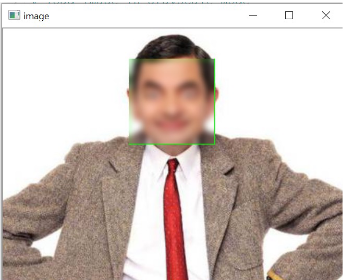
\includegraphics[width=0.8\linewidth]{images/example_blur_face.png}
    \caption{Minh họa hình ảnh đầu }
\end{figure}


\begin{verbatim}
import cv2
import numpy as np
import matplotlib.pyplot as plt

def blur_face_with_mean(image_path, face_coords, kernel_size=(35, 35)):ra
    """
    Làm mờ khuôn mặt trong ảnh sử dụng bộ lọc trung bình.

    Args:
        image_path (str): Đường dẫn đến ảnh.
        face_coords (tuple): Tọa độ (x, y, w, h) của khuôn mặt cần làm mờ.
        kernel_size (tuple): Kích thước của kernel (ví dụ: (35, 35)) để làm mờ.

    Returns:
        numpy.ndarray: Ảnh sau khi làm mờ khuôn mặt.
    """
    # Đọc ảnh
    image = cv2.imread(image_path)
    if image is None:
        print(f"Không thể đọc ảnh từ đường dẫn: {image_path}")
        return None

    # Chuyển đổi BGR sang RGB để hiển thị với matplotlib
    image_rgb = cv2.cvtColor(image, cv2.COLOR_BGR2RGB)
    
    # Tạo một bản sao của ảnh để xử lý
    output_image = image.copy()

    # Lấy tọa độ khuôn mặt
    x, y, w, h = face_coords

    # Cắt vùng khuôn mặt
    face_roi = output_image[y:y+h, x:x+w]

    # Áp dụng bộ lọc trung bình (mean filter) lên vùng khuôn mặt
    # cv2.blur() là một hàm thực hiện bộ lọc trung bình
    blurred_face_roi = cv2.blur(face_roi, kernel_size)

    # Đặt vùng khuôn mặt đã làm mờ trở lại ảnh gốc
    output_image[y:y+h, x:x+w] = blurred_face_roi

    # Chuyển đổi BGR sang RGB cho ảnh đầu ra để hiển thị
    output_image_rgb = cv2.cvtColor(output_image, cv2.COLOR_BGR2RGB)

    return image_rgb, output_image_rgb

original_img_rgb, blurred_img_rgb = blur_face_with_mean('image_e99a88.png', face_coordinates, kernel_size=(35, 35))

if original_img_rgb is not None and blurred_img_rgb is not None:
    plt.figure(figsize=(12, 6))

    plt.subplot(1, 2, 1)
    plt.imshow(original_img_rgb)
    plt.title('Ảnh Gốc')
    plt.axis('off')

    plt.subplot(1, 2, 2)
    plt.imshow(blurred_img_rgb)
    plt.title('Ảnh sau khi làm mờ khuôn mặt bằng Mean Filter')
    plt.axis('off')

    plt.show()
\end{verbatim}


\subsection{Ứng dụng của Median}

\textbf{Tính chất đặc biệt của Median:} Median ít bị ảnh hưởng bởi các outliers giúp khiến Median trở nên lý tưởng để khử nhiễu trắng đen bất thường trong ảnh khi nó có thể giúp mình lựa chọn giá trị trung bình dựa trên tần xuất xuất hiện của các điểm màu trong ảnh. 
\begin{itemize}
    \item Giả sử có một điểm ảnh trong vùng $3 \times 3$ có giá trị rất lớn (nhiễu trắng 255) hoặc rất nhỏ (nhiễu đen 0).
    \item Nếu dùng trung bình cộng (mean), giá trị nhiễu này sẽ ảnh hưởng đến kết quả.
    \item Nhưng nếu dùng median — là giá trị ở giữa sau khi sắp xếp — thì giá trị nhiễu nằm ở đầu/cuối danh sách nên sẽ bị bỏ qua.
\end{itemize}

\vspace{0.5em}
\textbf{Ví dụ minh họa:}

Giả sử ta có vùng ảnh nhỏ gồm 9 điểm ảnh có giá trị độ sáng như sau:

\[
[120, 122, 123, \boxed{255}, 124, 121, 123, 122, 120]
\]

Sau khi sắp xếp: 
\[
[120, 120, 121, 122, 122, 123, 123, 124, \boxed{255}]
\]

Median của vùng này là $122$, trong khi giá trị nhiễu $255$ bị loại bỏ khỏi trung tâm. Nhờ đó, ảnh sau khi xử lý median filter trở nên mượt mà hơn và loại bỏ được nhiễu đột ngột. Các bước xử lý ảnh sử dụng Median như sau, với ý tưởng là lướt 1 kernel có dạng ma trận vuông từ đầu đến cuối ảnh, với mỗi kernel tính Median và thay thế mọi giá trị trong kernel đó bằng Median. \\ 

\textbf{Thuật toán khử nhiễu:} Tạo kernel ma trận vuông $n \times n$ lướt từ trái sang phải, trên xuống dưới. Cho mỗi lần di chuyển.
\begin{enumerate}
\item Tính Median của kernel đó
\item Thay thế Median cho mọi giá trị trong kernel đó.
\end{enumerate}

\begin{figure}[H]
    \centering
    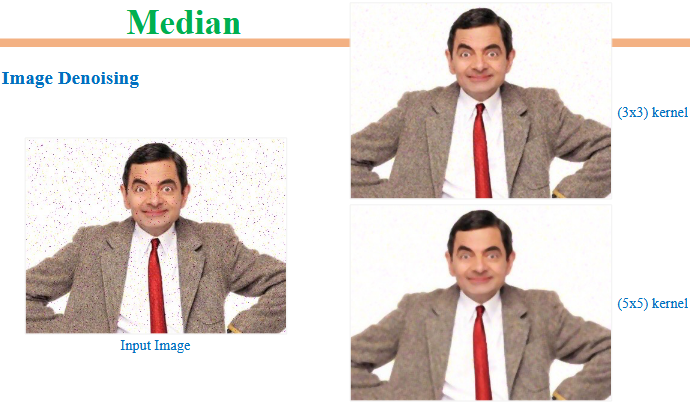
\includegraphics[width=0.9\linewidth]{images/median_noise.png} % Đảm bảo bạn đã lưu ảnh này (ví dụ: ảnh gốc, ảnh bị nhiễu, ảnh sau khử nhiễu)
    \caption{Minh họa ảnh gốc và ảnh đã khử nhiễu bằng Median Filter.}
\end{figure}

\begin{verbatim}
def startdenoise_image_with_median(image_path, kernel_size=5):
    """
    Khử nhiễu ảnh sử dụng bộ lọc trung vị.

    Args:
        image_path (str): Đường dẫn đến ảnh.
        kernel_size (int): Kích thước của kernel (phải là số lẻ, ví dụ: 3, 5, 7).

    Returns:
        tuple: (ảnh gốc RGB, ảnh đã khử nhiễu RGB) hoặc None nếu lỗi.
    """
    # Đọc ảnh
    image_bgr = cv2.imread(image_path)
    if image_bgr is None:
        print(f"Không thể đọc ảnh từ đường dẫn: {image_path}")
        return None

    # Chuyển đổi BGR sang RGB để hiển thị ảnh gốc
    original_image_rgb = cv2.cvtColor(image_bgr, cv2.COLOR_BGR2RGB)

    # Áp dụng bộ lọc trung vị
    # cv2.medianBlur hoạt động trực tiếp trên ảnh BGR hoặc grayscale
    denoised_image_bgr = cv2.medianBlur(image_bgr, kernel_size)

    # Chuyển ảnh đã khử nhiễu về RGB để hiển thị
    denoised_image_rgb = cv2.cvtColor(denoised_image_bgr, cv2.COLOR_BGR2RGB)

    return original_image_rgb, denoised_image_rgb

original_img_rgb, denoised_img_rgb = denoise_image_with_median('image.png', kernel_size=3)
 
plt.subplot(1, 2, 1)
plt.imshow(original_img_rgb)
plt.title('Ảnh Gốc (hoặc ảnh đã có nhiễu)')
plt.axis('off')

plt.subplot(1, 2, 2)
plt.imshow(denoised_img_rgb)
plt.title(f'Ảnh đã khử nhiễu bằng Median Filter (kernel={5})')
plt.axis('off')

plt.show()
\end{verbatim} \\ 

\subsection{Ứng dụng của Variance trong Phát hiện Cạnh (Edge Detection)}
\textbf{Ý tưởng chính:} Trong xử lý ảnh, khi xét một vùng nhỏ (patch hoặc kernel) quanh một điểm ảnh, nếu giá trị pixel trong vùng này thay đổi nhiều (có độ tương phản cao), thì phương sai và độ lệch chuẩn sẽ lớn. Ngược lại, nếu các pixel là $x_i$ có giá trị gần nhau (vùng phẳng), thì phương sai sẽ nhỏ. Do đó:
\[
\text{Std}(X) = \sqrt{\text{Var}(X)} 
\quad \text{Var}(X) = \frac{1}{n} \sum_{i=1}^{n} (x_i - \bar{x})^2
\quad \text{với } \bar{x} = \frac{1}{n} \sum_{i=1}^{n} x_i
\]

\begin{itemize}
\item Những vùng có \textbf{phương sai cao} thường là các cạnh, rìa, hoặc vùng có texture (chi tiết).
\item Những vùng có \textbf{phương sai thấp} thường là nền mịn, vùng trơn hoặc ít chi tiết.
\end{itemize}
Đây chính là cơ sở toán học để phát hiện biên trong ảnh bằng cách tính phương sai cục bộ.


\begin{figure}[H]
    \centering
    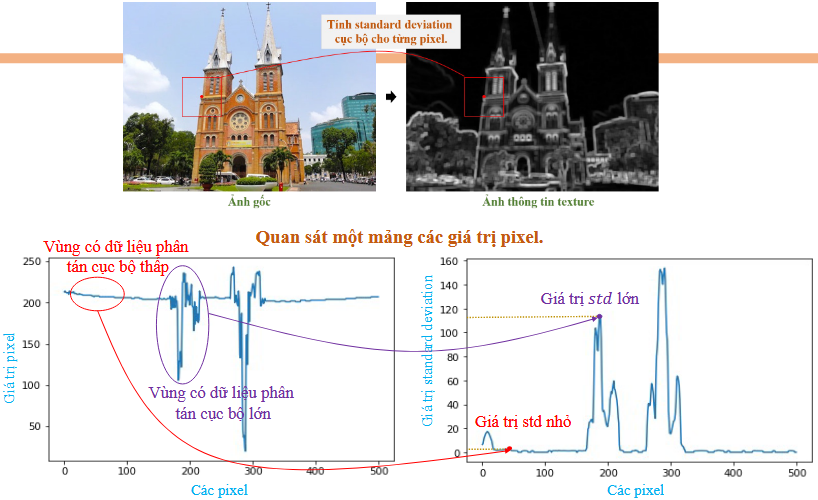
\includegraphics[width=0.85\linewidth]{images/variance_edge_detect.png} % thay bằng tên file thật nếu bạn có
    \caption{Tính phương sai cục bộ (local variance) để phát hiện biên trong ảnh.}
\end{figure}

\begin{figure}[H]
    \centering
    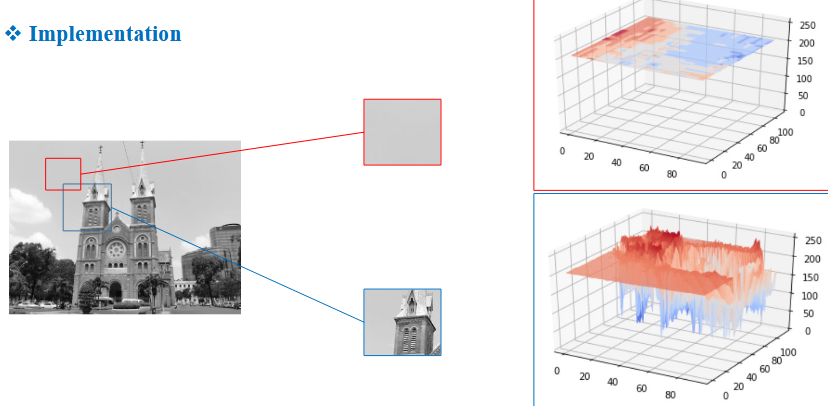
\includegraphics[width=0.8\linewidth]{images/variance_edge_detect3d.png} % ảnh 3D thể hiện độ biến thiên
    \caption{So sánh mặt phẳng 3D của hai vùng ảnh: vùng trơn (phương sai thấp) và vùng có chi tiết (phương sai cao).}
\end{figure}

\vspace{1em}


\textbf{Giải thích quy trình:}
\begin{enumerate}
    \item Ảnh màu được chuyển thành ảnh xám để đơn giản hóa xử lý.
    \item Mỗi điểm ảnh sẽ được xét trong một lân cận (kernel) có kích thước cố định (ví dụ: $7 \times 7$).
    \item Tính phương sai của giá trị pixel trong vùng lân cận này bằng hàm \texttt{np.std} (trong Python, standard deviation bình phương chính là variance).
    \item Kết quả là một bản đồ thể hiện độ biến thiên cường độ của từng vùng trong ảnh. Vùng nào có giá trị variance cao sẽ là vùng biên hoặc chứa nhiều texture.
    \item Ta có thể ngưỡng hóa để làm nổi bật các vùng có độ thay đổi lớn.
\end{enumerate}

\textbf{Code minh họa:}

\begin{verbatim}
import numpy as np
import cv2
from scipy.ndimage.filters import generic_filter

img = cv2.imread('img.jpg')
gray = cv2.cvtColor(img, cv2.COLOR_BGR2GRAY)

x = gray.astype('float')
# Tính standard deviation trong mỗi vùng 7x7
x_filter = generic_filter(x, np.std, size=7)

# Lọc bỏ vùng có giá trị std thấp (ngưỡng 20)
x_filter[x_filter < 20] = 0

# Phóng đại độ tương phản để hiển thị rõ biên
x_filter = x_filter * 2.5
cv2.imwrite('edge_output.jpg', x_filter)
\end{verbatim}

\begin{summarybox}
    \textbf{Từ ứng dụng trên ta nhận thấy:}
    \begin{itemize}
    \item Nhờ vào việc sử dụng phương sai, thuật toán có thể phát hiện các vùng biên rõ nét trong ảnh mà không cần tới các toán tử chuyên xử lý ảnh như Sobel hay Canny.
    \item Có thể áp dụng tiếp ngưỡng (thresholding) hoặc làm nét ảnh từ bản đồ phương sai này. 
    \end{itemize}
\end{summarybox} 


\section{Phần 9: Histogram và ứng dụng của nó}
\subsection{Histogram là gì?}
Histogram là biểu đồ thể hiện tần suất xuất hiện trong ảnh, giá trị của màu thường trải từ 0 đến 255 cho mỗi kênh màu. Cân bằng Histogram giúp tần số màu đồng đều, giúp người xem nhìn rõ hơn và hình ảnh rõ nét hơn.

\begin{figure}[H]
    \centering
    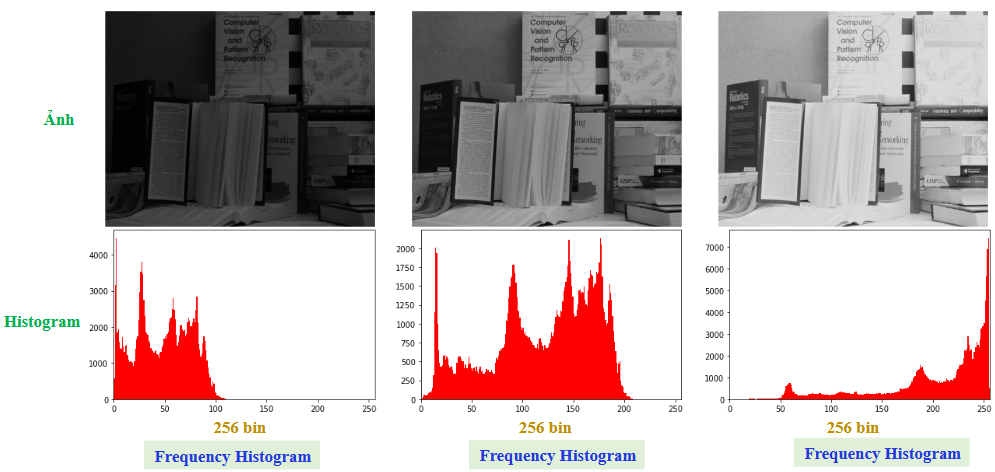
\includegraphics[width=0.8\linewidth]{images/histogram.png} % ảnh 3D thể hiện độ biến thiên
    \caption{Histogram của ảnh trong điều kiện sáng khác nhau}
\end{figure}

\textbf{Mô tả:}
\begin{itemize}
  \item Trục hoành: Các mức xám từ 0 đến 255. Giá trị của dải màu trên trục hoành gọi là bins, thông thường bins sẽ có 256 giá trị.
  \item Trục tung: Số lần xuất hiện tương ứng của mức xám đó trong toàn ảnh.
\end{itemize}

\subsection{Ứng dụng: Tăng độ tương phản bằng Histogram Equalization}

Histogram Equalization là một kỹ thuật dùng để \textbf{nâng cao độ tương phản} của ảnh. Ý tưởng chính là:

\begin{center}
\textit{Kéo phân bố của histogram sao cho gần xấp xỉ với phân bố đều (uniform distribution).}
\end{center}

Việc kéo histogram về gần phân bố đều giúp tận dụng toàn bộ dải màu thay vì cho dải màu của ảnh tụ lại 1 bên khiến ảnh sáng/tối nhiều hơn, nhờ đó ảnh sáng rõ hơn và tăng độ tương phản.



\vspace{0.2cm}
\begin{figure}[H]
    \centering
    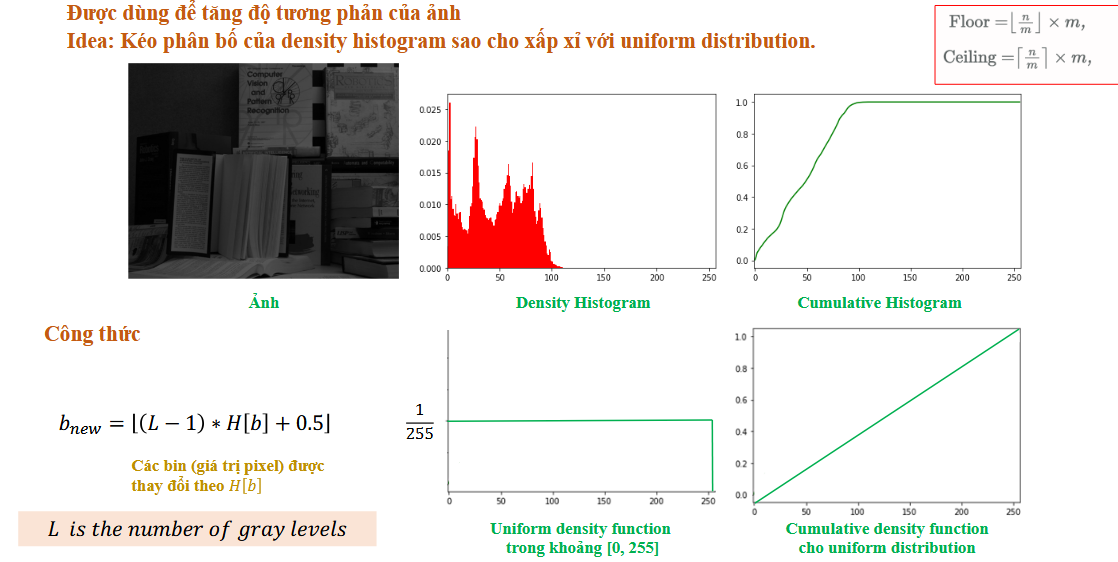
\includegraphics[width=0.8\linewidth]{images/he_idea.png} % ảnh 3D thể hiện độ biến thiên
    \caption{Ý tưởng tăng độ tương phản của ảnh}
\end{figure}

\noindent\textbf{Chi tiết từng bước giúp tăng độ tương phản:}

\begin{enumerate}
  \item \textbf{Phân tích histogram ban đầu:} Histogram của ảnh gốc thường bị lệch – ví dụ tập trung nhiều ở mức xám thấp (ảnh tối) hoặc mức xám cao (ảnh sáng chói). Điều này khiến ảnh thiếu độ tương phản, các chi tiết bị mờ.

  \item \textbf{Chuẩn hóa histogram thành phân bố xác suất (PDF):} Mỗi mức xám được chia cho tổng số pixel để trở thành xác suất xuất hiện. Bước này giúp chuyển đổi histogram về dạng có thể so sánh và tính tích lũy.

  \item \textbf{Tính hàm phân phối tích lũy (CDF):} Cộng dồn xác suất từ mức xám thấp đến mức xám hiện tại. Giá trị CDF sẽ dao động từ 0 đến 1. Đây chính là hàm ánh xạ mức xám.

  \item \textbf{Ánh xạ mức xám mới:} Mỗi mức xám $b$ ban đầu sẽ được chuyển sang mức mới $b_{\text{new}}$ theo công thức:
  \[
  b_{\text{new}} = \left\lfloor (L - 1) \cdot H[b] + 0.5 \right\rfloor
  \]

Trong đó:
\begin{itemize}
  \item $L$ là số mức xám (thường là 256, trừ 1 để về ).
  \item $H[b]$ là giá trị CDF tại mức xám bin $b$ (chuẩn hóa về [0,1]).
  \item $b_{\text{new}}$ là mức xám mới sau khi ánh xạ.
\end{itemize}
 Việc này giúp kéo các mức xám về đều hơn trên toàn dải $[0, 255]$.

  \item \textbf{Tăng độ tương phản:} 
  Khi histogram ban đầu bị dồn về một phía (ví dụ: tối nhiều), việc trải đều các giá trị mức xám thông qua CDF giúp:
  \begin{itemize}
    \item Làm rõ các chi tiết bị ẩn trong vùng tối hoặc sáng.
    \item Mở rộng dải động (dynamic range) của ảnh.
    \item Ảnh trở nên "sống động" và dễ xử lý trong các bước nhận dạng/phân tích sau đó.
  \end{itemize}
\end{enumerate}

\section{Phần 10 Mở rộng: Cài đặt Histogram sử dụng numpy}

\end{document}